\documentclass[11pt,a4paper]{report}
\usepackage[textwidth=37em,vmargin=30mm]{geometry}
\usepackage{calc,xunicode,amsmath,amssymb,paralist,enumitem,tabu,booktabs,datetime2,xeCJK,xeCJKfntef,listings}
\usepackage{tocloft,fancyhdr,tcolorbox,xcolor,graphicx,eso-pic,xltxtra,xelatexemoji}

\newcommand{\envyear}[0]{2025}
\newcommand{\envdatestr}[0]{2025-06-18}
\newcommand{\envfinaldir}[0]{webdb/2025/20250618/final}

\usepackage[hidelinks]{hyperref}
\hypersetup{
    colorlinks=false,
    pdfpagemode=FullScreen,
    pdftitle={Web Digest - \envdatestr}
}

\setlength{\cftbeforechapskip}{10pt}
\renewcommand{\cftchapfont}{\rmfamily\bfseries\large\raggedright}
\setlength{\cftbeforesecskip}{2pt}
\renewcommand{\cftsecfont}{\sffamily\small\raggedright}

\setdefaultleftmargin{2em}{2em}{1em}{1em}{1em}{1em}

\usepackage{xeCJK,xeCJKfntef}
\xeCJKsetup{PunctStyle=plain,RubberPunctSkip=false,CJKglue=\strut\hskip 0pt plus 0.1em minus 0.05em,CJKecglue=\strut\hskip 0.22em plus 0.2em}
\XeTeXlinebreaklocale "zh"
\XeTeXlinebreakskip = 0pt


\setmainfont{Brygada 1918}
\setromanfont{Brygada 1918}
\setsansfont{IBM Plex Sans}
\setmonofont{JetBrains Mono NL}
\setCJKmainfont{Noto Serif CJK SC}
\setCJKromanfont{Noto Serif CJK SC}
\setCJKsansfont{Noto Sans CJK SC}
\setCJKmonofont{Noto Sans CJK SC}

\setlength{\parindent}{0pt}
\setlength{\parskip}{8pt}
\linespread{1.15}

\lstset{
	basicstyle=\ttfamily\footnotesize,
	numbersep=5pt,
	backgroundcolor=\color{black!5},
	showspaces=false,
	showstringspaces=false,
	showtabs=false,
	tabsize=2,
	captionpos=b,
	breaklines=true,
	breakatwhitespace=true,
	breakautoindent=true,
	linewidth=\textwidth
}






\newcommand{\coverpic}[2]{
    % argv: itemurl, authorname
    Cover photo by #2~~(\href{#1}{#1})
}
\newcommand{\makeheader}[0]{
    \begin{titlepage}
        % \newgeometry{hmargin=15mm,tmargin=21mm,bmargin=12mm}
        \begin{center}
            
            \rmfamily\scshape
            \fontspec{BaskervilleF}
            \fontspec{Old Standard}
            \fontsize{59pt}{70pt}\selectfont
            WEB\hfill DIGEST
            
            \vfill
            % \vskip 30pt
            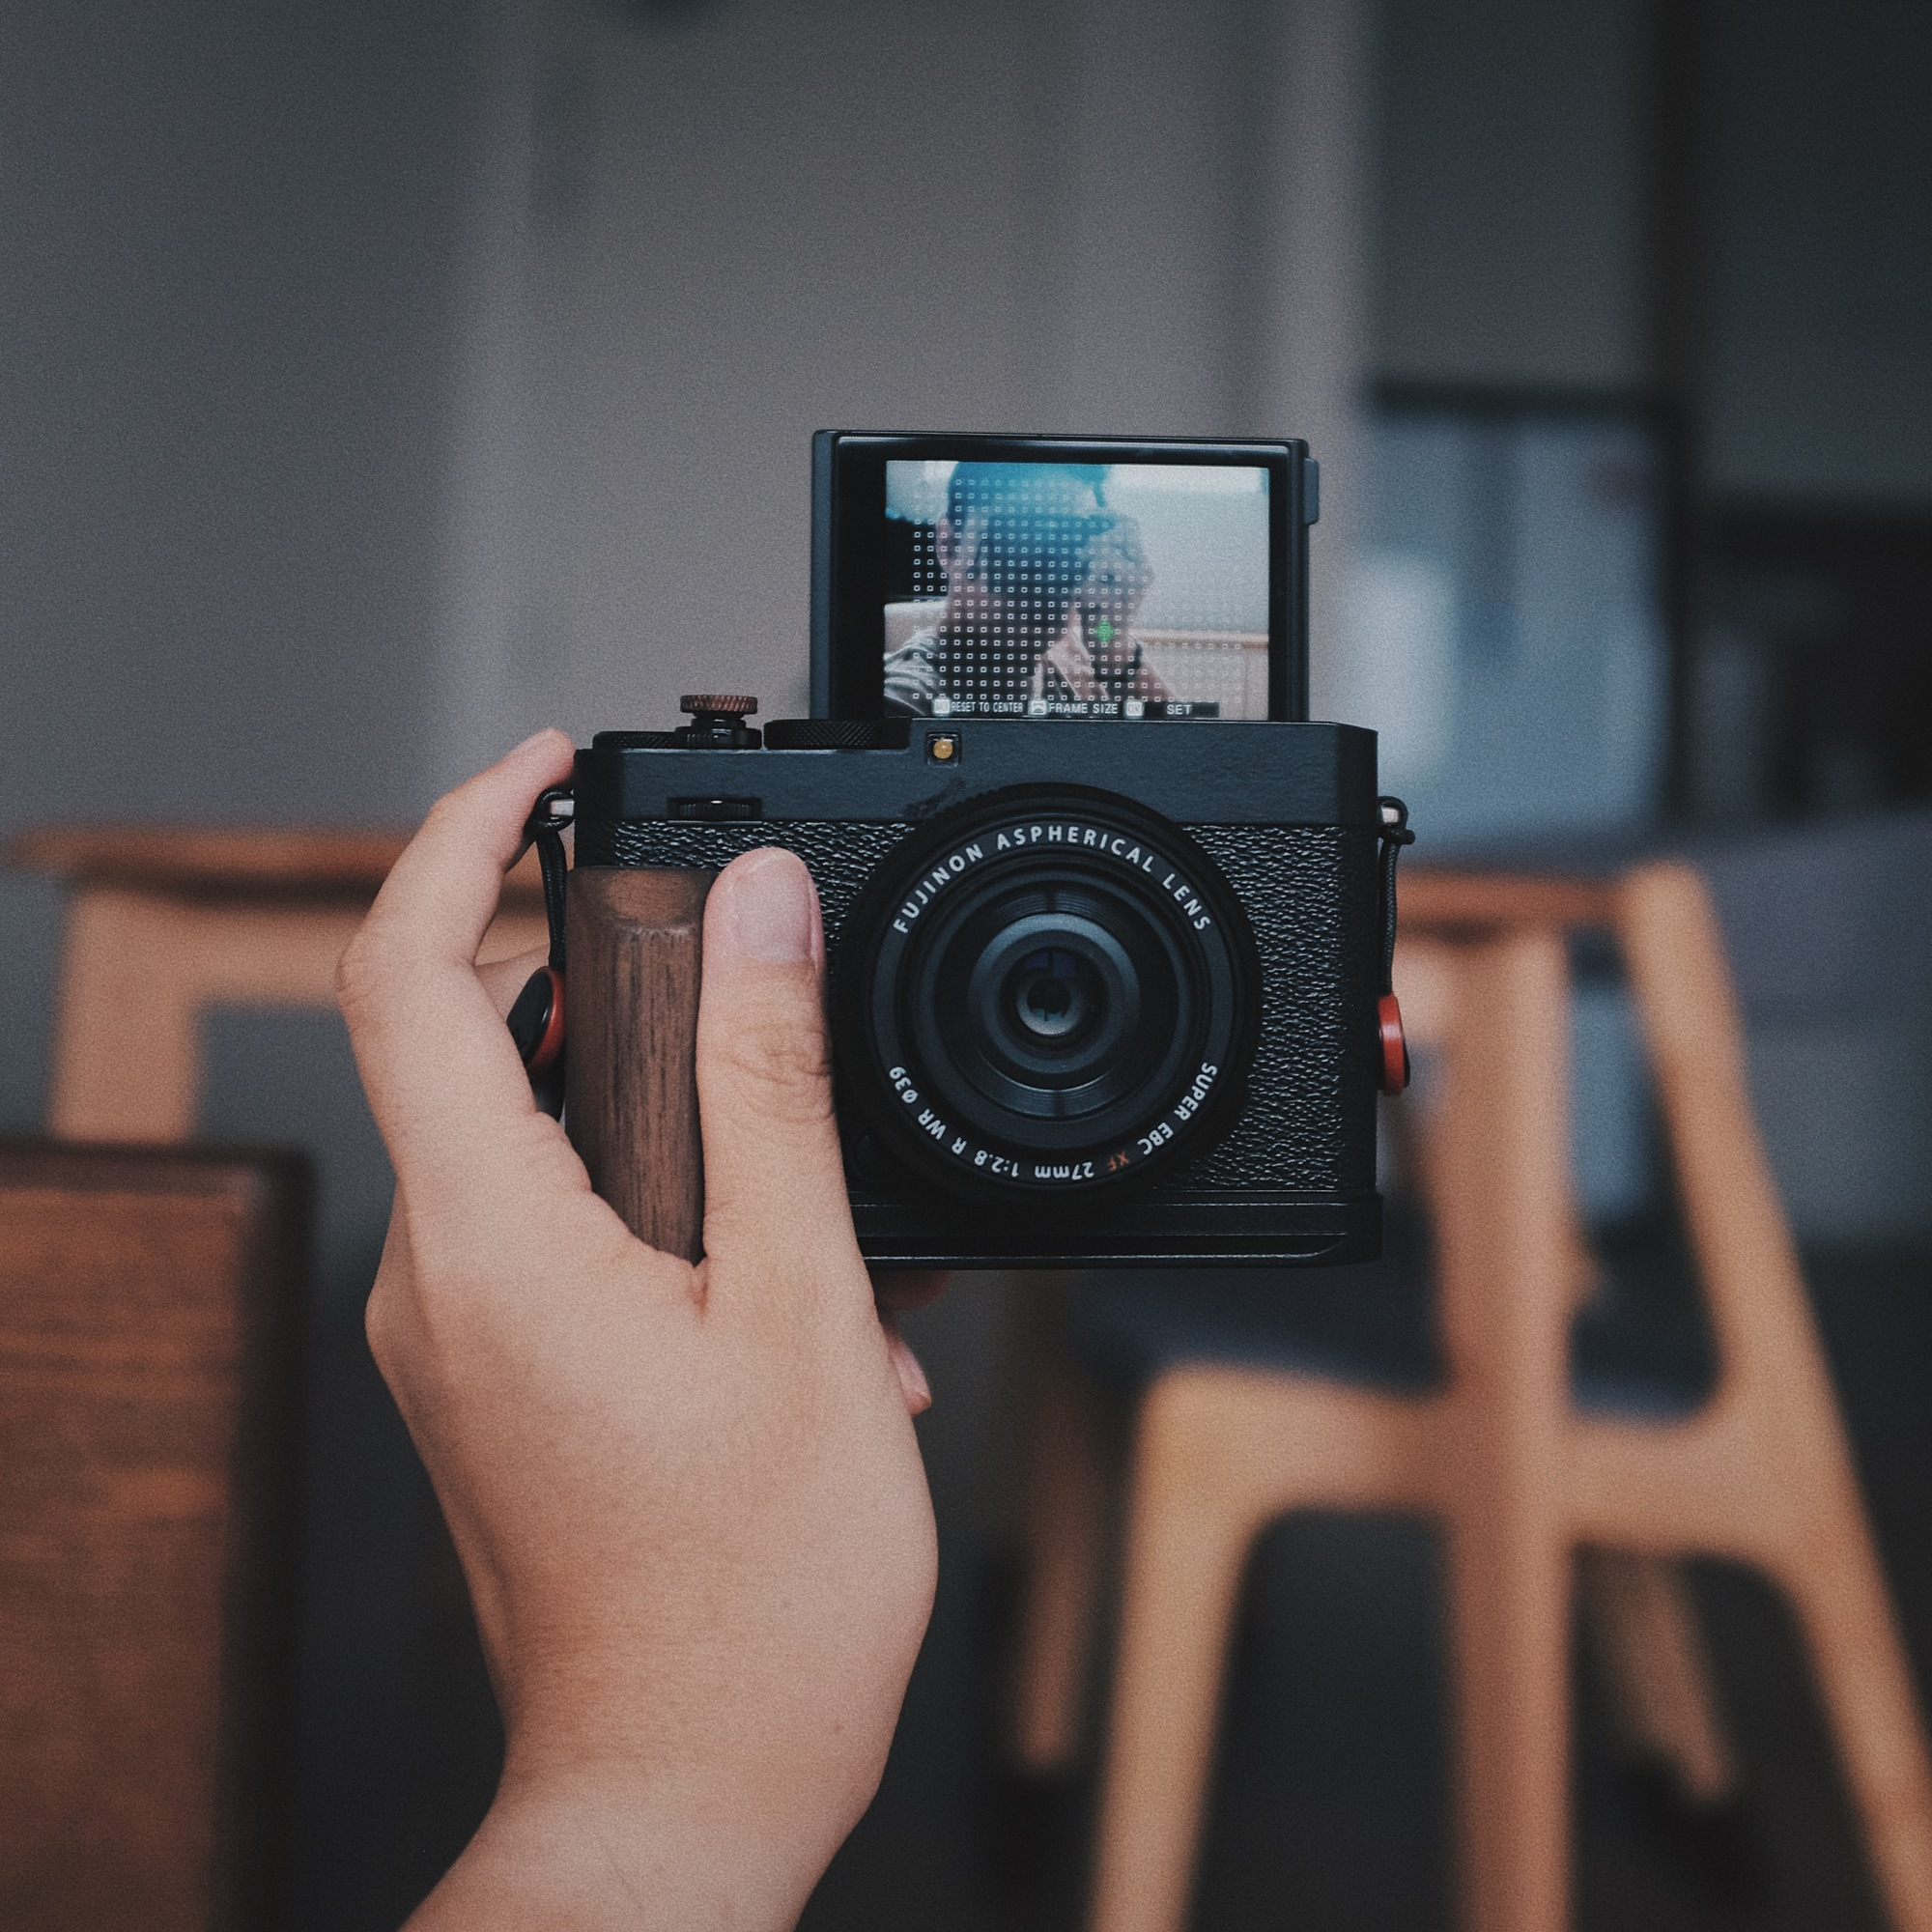
\includegraphics[width=\linewidth]{\envfinaldir/coverpic-prod.jpg}\par
            % \vskip 30pt
            \vfill

            \normalsize\rmfamily\scshape
            \copyright{} The Web Digest Project \hfill\large \envdatestr
        \end{center}
    \end{titlepage}
    % \restoregeometry
}
\newcommand{\simplehref}[1]{%
    \textcolor{blue!80!green}{\href{#1}{#1}}%
}
\renewcommand{\contentsname}{\center\Huge\sffamily\bfseries Contents\par\vskip 20pt}
\newcounter{ipartcounter}
\setcounter{ipartcounter}{0}
\newcommand{\ipart}[1]{
    % \vskip 20pt
    \clearpage
    \stepcounter{ipartcounter}
    \phantomsection
    \addcontentsline{toc}{chapter}{#1}
    % \begin{center}
    %     \Huge
    %     \sffamily\bfseries
    %     #1
    % \end{center}
    % \vskip 20pt plus 7pt
}
\newcounter{ichaptercounter}
\setcounter{ichaptercounter}{0}
\newcommand{\ichapter}[1]{
    % \vskip 20pt
    \clearpage
    \stepcounter{ichaptercounter}
    \phantomsection
    \addcontentsline{toc}{section}{\numberline{\arabic{ichaptercounter}}#1}
    \begin{center}
        \Huge
        \sffamily\bfseries
        #1
    \end{center}
    \vskip 20pt plus 7pt
}
\newcommand{\entrytitlefont}[1]{\subsection*{\raggedright\Large\sffamily\bfseries#1}}
\newcommand{\entryitemGeneric}[2]{
    % argv: title, url
    \parbox{\linewidth}{
        \entrytitlefont{#1}\par\vskip 5pt
        \footnotesize\ttfamily\mdseries
        \simplehref{#2}
    }\vskip 11pt plus 11pt minus 1pt
}
\newcommand{\entryitemGithub}[3]{
    % argv: title, url, desc
    \parbox{\linewidth}{
        \entrytitlefont{#1}\par\vskip 5pt
        \footnotesize\ttfamily\mdseries
        \simplehref{#2}\par\vskip 5pt
        \small\rmfamily\mdseries#3
    }\vskip 11pt plus 11pt minus 1pt
}
\newcommand{\entryitemAp}[3]{
    % argv: title, url, desc
    \parbox{\linewidth}{
        \entrytitlefont{#1}\par\vskip 5pt
        \footnotesize\ttfamily\mdseries
        \simplehref{#2}\par\vskip 5pt
        \small\rmfamily\mdseries#3
    }\vskip 11pt plus 11pt minus 1pt
}
\newcommand{\entryitemHackernews}[3]{
    % argv: title, hnurl, rawurl
    % \parbox{\linewidth}{
    %     \entrytitlefont{#1}\par\vskip 5pt
    %     \footnotesize\ttfamily\mdseries
    %     \simplehref{#3}\par
    %     \textcolor{black!50}{\href{#2}{#2}}
    % }\vskip 11pt plus 11pt minus 1pt
    \begin{minipage}{\linewidth}
            \entrytitlefont{#1}\par\vskip 5pt
            \footnotesize\ttfamily\mdseries
            \simplehref{#3}\par
            \textcolor{black!50}{\href{#2}{#2}}
    \end{minipage}\par\vskip 11pt plus 11pt minus 1pt
}







\begin{document}

\makeheader

\tableofcontents\clearpage




\ipart{Developers}
\ichapter{Hacker News}
\entryitemTwoLinks{The Grug Brained Developer (2022)}{https://news.ycombinator.com/item?id=44303542}{https://grugbrain.dev/}

\entryitemTwoLinks{Bzip2 crate switches from C to 100\% Rust}{https://news.ycombinator.com/item?id=44303361}{https://trifectatech.org/blog/bzip2-crate-switches-from-c-to-rust/}

\entryitemTwoLinks{Iran asks its people to delete WhatsApp from their devices}{https://news.ycombinator.com/item?id=44302752}{https://apnews.com/article/iran-whatsapp-meta-israel-d9e6fe43280123c9963802e6f10ac8d1}

\entryitemTwoLinks{Building Effective AI Agents}{https://news.ycombinator.com/item?id=44301809}{https://www.anthropic.com/engineering/building-effective-agents}

\entryitemTwoLinks{Resurrecting a dead torrent tracker and finding 3M peers}{https://news.ycombinator.com/item?id=44301686}{https://kianbradley.com/2025/06/15/resurrecting-a-dead-tracker.html}

\entryitemTwoLinks{Brad Lander detained by masked federal agents inside immigration court}{https://news.ycombinator.com/item?id=44301501}{https://www.thecity.nyc/2025/06/17/brad-lander-arrest-ice-immigration-court/}

\entryitemTwoLinks{Miscalculation by Spanish power grid operator REE contributed to blackout}{https://news.ycombinator.com/item?id=44301186}{https://www.reuters.com/business/energy/investigation-into-spains-april-28-blackout-shows-no-evidence-cyberattack-2025-06-17/}

\entryitemTwoLinks{Tesla Robotaxi launch is a dangerous game of smoke and mirrors}{https://news.ycombinator.com/item?id=44300727}{https://electrek.co/2025/06/16/tesla-robotaxi-launch-dangerous-game-smoke-mirrors/}

\entryitemTwoLinks{Making 2.5 Flash and 2.5 Pro GA, and introducing Gemini 2.5 Flash-Lite}{https://news.ycombinator.com/item?id=44300717}{https://blog.google/products/gemini/gemini-2-5-model-family-expands/}

\entryitemTwoLinks{Honda conducts successful launch and landing of experimental reusable rocket}{https://news.ycombinator.com/item?id=44300102}{https://global.honda/en/topics/2025/c\_2025-06-17ceng.html}

\entryitemTwoLinks{Now might be the best time to learn software development}{https://news.ycombinator.com/item?id=44299979}{https://substack.com/home/post/p-165655726}

\entryitemTwoLinks{Why JPEGs still rule the web (2024)}{https://news.ycombinator.com/item?id=44299970}{https://spectrum.ieee.org/jpeg-image-format-history}

\entryitemTwoLinks{O3 Turns Pro}{https://news.ycombinator.com/item?id=44299947}{https://thezvi.substack.com/p/o3-turns-pro}

\entryitemTwoLinks{Should we design for iffy internet?}{https://news.ycombinator.com/item?id=44298656}{https://bytes.zone/posts/should-we-design-for-iffy-internet/}

\entryitemTwoLinks{No Hello}{https://news.ycombinator.com/item?id=44297431}{https://nohello.net/en/}

\entryitemTwoLinks{The magic of through running}{https://news.ycombinator.com/item?id=44297045}{https://www.worksinprogress.news/p/the-magic-of-through-running}

\entryitemTwoLinks{Accumulation of Cognitive Debt When Using an AI Assistant for Essay Writing Task}{https://news.ycombinator.com/item?id=44296711}{https://www.brainonllm.com/}

\entryitemTwoLinks{Fossify – A suite of open-source, ad-free apps}{https://news.ycombinator.com/item?id=44296564}{https://github.com/FossifyOrg}

\entryitemTwoLinks{Fun with Telnet (2024)}{https://news.ycombinator.com/item?id=44295925}{https://brandonrozek.com/blog/fun-with-telnet/}

\entryitemTwoLinks{Show HN: I recreated 90s Mode X demoscene effects in JavaScript and Canvas}{https://news.ycombinator.com/item?id=44295667}{https://jdfio.com/pages-output/demos/x-mode/}


\ipart{Developers~~~~(zh-Hans)}
\ichapter{Solidot}
\entryitemGeneric{\hskip 0pt{}科学家创造出一种致命真菌去对抗蚊子}{https://www.solidot.org/story?sid=81582}

\entryitemGeneric{\hskip 0pt{}研究人员创造出第一种完全可验证的真随机数生成器}{https://www.solidot.org/story?sid=81581}

\entryitemGeneric{\hskip 0pt{}KDE Plasma 6.4 释出}{https://www.solidot.org/story?sid=81580}

\entryitemGeneric{\hskip 0pt{}特朗普集团宣布 499 美元智能手机}{https://www.solidot.org/story?sid=81579}

\entryitemGeneric{\hskip 0pt{}美国最主要的新闻来源如今是社交媒体}{https://www.solidot.org/story?sid=81578}

\entryitemGeneric{\hskip 0pt{}英特尔将裁减 15\%-20\% 的芯片工厂员工}{https://www.solidot.org/story?sid=81577}

\entryitemGeneric{\hskip 0pt{}OpenAI 和微软之间的紧张关系加剧 }{https://www.solidot.org/story?sid=81576}

\entryitemGeneric{\hskip 0pt{}Nexus Mods 创始人卸任}{https://www.solidot.org/story?sid=81575}

\entryitemGeneric{\hskip 0pt{}大部分重子物质藏身于星际之间}{https://www.solidot.org/story?sid=81574}

\entryitemGeneric{\hskip 0pt{}LibreOffice 25.8 将停止支持 Windows 7 和 8/8.1}{https://www.solidot.org/story?sid=81573}

\entryitemGeneric{\hskip 0pt{}17 岁学生让无人机能像鱼鹰一样飞行}{https://www.solidot.org/story?sid=81572}

\entryitemGeneric{\hskip 0pt{}AI教父辛顿最新访谈:在个性化算法时代,人类的共同体验消失了,数字智能必然超越生物智能,但20\%的灭绝概率正被忽视}{https://www.solidot.org/story?sid=81571}

\entryitemGeneric{\hskip 0pt{}英国连锁店的面部识别系统错误识别一位女性为小偷}{https://www.solidot.org/story?sid=81569}

\entryitemGeneric{\hskip 0pt{}纽约州开始要求雇主披露裁员是否是 AI 导致的}{https://www.solidot.org/story?sid=81568}

\entryitemGeneric{\hskip 0pt{}YouTube 和 Spotify 出现假专辑和 AI 生成音乐 }{https://www.solidot.org/story?sid=81567}

\entryitemGeneric{\hskip 0pt{}Meta 的大模型 Llama 3.1 能回忆《哈利波特》第一部 42\% 的内容 }{https://www.solidot.org/story?sid=81566}

\entryitemGeneric{\hskip 0pt{}X.Org Server 项目回滚了大量代码}{https://www.solidot.org/story?sid=81565}

\entryitemGeneric{\hskip 0pt{}女孩的数学表现从上学起开始落后}{https://www.solidot.org/story?sid=81564}

\entryitemGeneric{\hskip 0pt{}吃水果和蔬菜与高质量睡眠相关}{https://www.solidot.org/story?sid=81563}

\entryitemGeneric{\hskip 0pt{}饥饿细菌会杀死并吞食其邻居}{https://www.solidot.org/story?sid=81562}\ichapter{V2EX}
\entryitemGeneric{\hskip 0pt{}[分享发现] 推荐一个代码字体 Martian Mono}{https://www.v2ex.com/t/1139313}

\entryitemGeneric{\hskip 0pt{}[分享创造] 第 137 期-偷懒爱好者周刊 25/06/18}{https://www.v2ex.com/t/1139312}

\entryitemGeneric{\hskip 0pt{}[iPhone] 请问 grow app 可以用家庭组共享吗?}{https://www.v2ex.com/t/1139311}

\entryitemGeneric{\hskip 0pt{}[创业组队] 寻找志同道合的技术合伙人|优质项目启动中}{https://www.v2ex.com/t/1139310}

\entryitemGeneric{\hskip 0pt{}[Linux] Fedora Silverblue 上怎样丝滑地使用 IDE}{https://www.v2ex.com/t/1139309}

\entryitemGeneric{\hskip 0pt{}[问与答] cursor 现在是不限制使用量了么?}{https://www.v2ex.com/t/1139308}

\entryitemGeneric{\hskip 0pt{}[Apple] 苹果 AI(Apple Intelligence)都发布一年过去了, 国行什么时候能用上}{https://www.v2ex.com/t/1139307}

\entryitemGeneric{\hskip 0pt{}[问与答] 想装个 5080+9800X3D 的主机,帮看看这几个配置哪个合适}{https://www.v2ex.com/t/1139306}

\entryitemGeneric{\hskip 0pt{}[Django] 大家学习编程做项目的时候一开始会容易卡壳吗?比如我今天一个下午才弄出来了博客当中的文章评论加回复功能,有时候会因为一个小点卡壳,稍微复杂点的逻辑就感觉脑子不够用,甚至是给 html 的 div 取变量名的时候脑子也会不够}{https://www.v2ex.com/t/1139305}

\entryitemGeneric{\hskip 0pt{}[酷工作] 汇丰银行内推 [广州 西安 上海]}{https://www.v2ex.com/t/1139304}

\entryitemGeneric{\hskip 0pt{}[程序员] cursor pro 无法使用 cluade4.0 了}{https://www.v2ex.com/t/1139300}

\entryitemGeneric{\hskip 0pt{}[macOS] 关于升级 macOS 26 后 LaunchPad 如何调回来}{https://www.v2ex.com/t/1139298}

\entryitemGeneric{\hskip 0pt{}[站长] 移动机房托管网络质量太差了吧}{https://www.v2ex.com/t/1139297}

\entryitemGeneric{\hskip 0pt{}[职场话题] 工作中,你一直循环的歌单}{https://www.v2ex.com/t/1139296}

\entryitemGeneric{\hskip 0pt{}[程序员] https://marketplace.visualstudio.com 这个网站是不是挂掉了?}{https://www.v2ex.com/t/1139295}

\entryitemGeneric{\hskip 0pt{}[问与答] 请问有没有办法带一套 3.2V 大容量(60Wh 以上,越大越好)锂电池(系统)上飞机}{https://www.v2ex.com/t/1139294}

\entryitemGeneric{\hskip 0pt{}[职场话题] 新公司 2 个月,有点迷茫}{https://www.v2ex.com/t/1139293}

\entryitemGeneric{\hskip 0pt{}[程序员] 主打一个免费 cursor 混搭 gemini 2.5 flash/deepseek v3.1 写代码}{https://www.v2ex.com/t/1139292}

\entryitemGeneric{\hskip 0pt{}[职场话题] 群里小伙伴们: 投诉我 vx 对群里的人有什么益处尼?}{https://www.v2ex.com/t/1139290}

\entryitemGeneric{\hskip 0pt{}[物联网] 米家设备实际连上 WiFi 但米家 App 报告失败}{https://www.v2ex.com/t/1139289}

\entryitemGeneric{\hskip 0pt{}[分享创造] 做了一个自己趁手的节省 cursor request 小工具, 已经完全用 agent 代替 ask 模式了。}{https://www.v2ex.com/t/1139288}

\entryitemGeneric{\hskip 0pt{}[摄影] 佳能的相机,用起来怎么样?}{https://www.v2ex.com/t/1139287}

\entryitemGeneric{\hskip 0pt{}[分享发现] Cursor Pro 从 500 次变成了不限制了, Vibe Coding 战争正在加剧}{https://www.v2ex.com/t/1139285}

\entryitemGeneric{\hskip 0pt{}[YouTube] 分享一个一键提取 YouTube 视频封面的线上下载工具,支持 Youtube 视频全格式链接}{https://www.v2ex.com/t/1139282}

\entryitemGeneric{\hskip 0pt{}[分享创造] 手把手教你免费生成 Labubu 潮玩!无需抢购,轻松实现 Labubu 自由}{https://www.v2ex.com/t/1139281}

\entryitemGeneric{\hskip 0pt{}[分享创造] 为什么股票软件都是需要一个个点击去才能看到走势图?我做了一个网站一进去就可以看到所有走势图}{https://www.v2ex.com/t/1139280}

\entryitemGeneric{\hskip 0pt{}[分享发现] 免费体验 CloudFlare 的企业套餐,永久免费二级域}{https://www.v2ex.com/t/1139279}

\entryitemGeneric{\hskip 0pt{}[分享创造] 写了个对话导出增强插件,支持 deepseek 和豆包,后续有人用再扩展别的}{https://www.v2ex.com/t/1139278}

\entryitemGeneric{\hskip 0pt{}[NAS] 用硬盘柜+Mac Mini 代替 NAS 是否靠谱}{https://www.v2ex.com/t/1139277}

\entryitemGeneric{\hskip 0pt{}[程序员] 实际的业务中,图数据库常见吗}{https://www.v2ex.com/t/1139275}

\entryitemGeneric{\hskip 0pt{}[推广] 需要天翼云折扣优惠的看过来~}{https://www.v2ex.com/t/1139274}

\entryitemGeneric{\hskip 0pt{}[Surge] surge 的远端 domain set 会自动更新吗}{https://www.v2ex.com/t/1139272}

\entryitemGeneric{\hskip 0pt{}[职场话题] 30 岁之后,开发转 PM 是不是必须的呢}{https://www.v2ex.com/t/1139271}

\entryitemGeneric{\hskip 0pt{}[职场话题] 拿礼包 or 一人坚守,请君赐我一策}{https://www.v2ex.com/t/1139270}

\entryitemGeneric{\hskip 0pt{}[问与答] Mac 安装软件的``已损坏,无法打开。 您应该将它移到废纸篓''这个怎么解决呢}{https://www.v2ex.com/t/1139269}

\entryitemGeneric{\hskip 0pt{}[酷工作] [北京望京] 20-35k 招聘 Flutter 开发工程师}{https://www.v2ex.com/t/1139266}

\entryitemGeneric{\hskip 0pt{}[宽带症候群] 武汉电信 美好家 5g 179 100GB 800 分钟 1+9=10 卡共享}{https://www.v2ex.com/t/1139265}

\entryitemGeneric{\hskip 0pt{}[游戏主机] 想买一套 5080 的主机 帮看下这个配置行不}{https://www.v2ex.com/t/1139264}

\entryitemGeneric{\hskip 0pt{}[问与答] 上海 iPhone 手机屏幕维修有靠谱的店铺吗}{https://www.v2ex.com/t/1139262}

\entryitemGeneric{\hskip 0pt{}[游戏开发] 学了两年多 Unity,昨天体验了下虚幻 5,也太丝滑了,为什么 Unity 会这么卡?}{https://www.v2ex.com/t/1139261}

\entryitemGeneric{\hskip 0pt{}[问与答] 是否需要这样一个 [域名] 相关网站}{https://www.v2ex.com/t/1139260}

\entryitemGeneric{\hskip 0pt{}[求职] 求一份前端暑期实习, 211 本硕,熟练使用 Vue}{https://www.v2ex.com/t/1139258}

\entryitemGeneric{\hskip 0pt{}[Apple] 2025 年 macbookpro M 怎么读写 ntfs 的 upan?请各位大佬赐教,免费开源是最好。}{https://www.v2ex.com/t/1139257}

\entryitemGeneric{\hskip 0pt{}[问与答] 4K 屏幕 200\%缩放下的字体问题}{https://www.v2ex.com/t/1139256}

\entryitemGeneric{\hskip 0pt{}[分享发现] 🌟 分享一个无痛学习英语的工具}{https://www.v2ex.com/t/1139255}

\entryitemGeneric{\hskip 0pt{}[职场话题] 骑驴找马,在飞书视频面试登陆了账号,会被目前公司知道吗?}{https://www.v2ex.com/t/1139254}

\entryitemGeneric{\hskip 0pt{}[问与答] 自动化抓取银行余额变动}{https://www.v2ex.com/t/1139252}

\entryitemGeneric{\hskip 0pt{}[Nintendo Switch] Nintendo Switch Online 高级版(+扩充包)发车}{https://www.v2ex.com/t/1139251}

\entryitemGeneric{\hskip 0pt{}[加密货币] 第一次玩合约,刚开始赚了 10 万,然后 20 分钟不到就全部没了,爆仓了}{https://www.v2ex.com/t/1139250}

\entryitemGeneric{\hskip 0pt{}[分享创造] 我的工资 - 有点鸡肋}{https://www.v2ex.com/t/1139249}


\ipart{Generic News}
\ichapter{联合早报}
\entryitemWithDescription{杨丹旭:关税战中找定力}{https://www.zaobao.com/news/china/story20250617-6814940}{中美伦敦经贸磋商后,美国媒体彭博社发表了一篇评论文章,概括中美对待这场贸易争端截然不同的两种思维:美国领导人急于出成果,而中国领导人专注打长线战。 评论指出,中美伦敦经贸磋商后,美国总统特朗普对谈判结果大加赞赏,不仅在社交媒体上宣布,已与中国达成``协议'',来自中国的关键磁铁将恢复供应,美国也承诺会放宽对中国学生的签证限制……}

\entryitemWithDescription{中国5月消费显著回升达6.4\%成经济亮点 工业与房地产仍负重前行}{https://www.zaobao.com/news/china/story20250616-6807120}{在中美贸易战阴霾下,中国5月消费创下6.4\%的超预期增长,为一年半来最高增速,部分缓解了美国加征关税对中国增长的压力,但工业和房地产市场依然在负重前行。 中国官方表示,5月消费增长得益于多重利好因素叠加,包括``五一''\,``端午''假日消费、消费品以旧换新政策的带动,以及中国电商今年提早启动``618''大促等。分析预计北京将继续通过补贴政策刺激消费,并有可能出台新措施以稳定房地产市场……}

\entryitemWithDescription{福建舰下水三周年 中国官媒称三航母时代即将到来}{https://www.zaobao.com/news/china/story20250616-6811085}{(北京/香港综合讯)中国官媒透露,中国第三艘航母福建舰的海试工作正按计划稳步推进,海军三航母时代即将到来。有学者分析,福建舰服役后可直接压缩台军预警时间。 据央视新闻节目《军情时间到》上星期六(6月14日)报道,福建舰迎来下水三周年之际,相关建设和海事工作不断推进。福建舰入列后,将大幅提升中国海军近海防御和远海护卫作战的能力,中国海军也将正式进入三航母时代……}

\entryitemWithDescription{赖清德吁台美共同生产研发军备}{https://www.zaobao.com/news/china/story20250616-6811831}{(台北综合讯)台湾总统赖清德星期一(6月16日)接见到访的美国联邦众议员时表示,希望台美安全合作从军购迈向``共同生产、共同研发''伙伴关系……}

\entryitemWithDescription{夏宝龙据报星期三访港 将与八所大学高层闭门座谈}{https://www.zaobao.com/news/china/story20250616-6812113}{(香港综合讯)香港国安法实施五周年之际,中国国务院港澳事务办公室主任夏宝龙据报星期三(6月18日)起赴港调研五天。 香港《信报》星期一(16日)引述消息称,夏宝龙访港日期基本敲定在6月18日至22日,五天行程紧凑,除了出席星期六(21日)举办的``香港国安法公布实施五周年论坛''外,他还将到地方了解民情、与商界领袖座谈……}

\entryitemWithDescription{香港今年将提前发表《施政报告》 学者预计重点是发展经济}{https://www.zaobao.com/news/china/story20250616-6810243}{香港新一届立法会选举将在今年底举行,特区政府为此将首次提前在9月发表新一份《施政报告》。受访学者预计,由于香港经济不景气,今年《施政报告》除了继续加强国家安全领域的建设,也会着力提出发展经济的措施。 港府星期一(6月16日)宣布,行政长官李家超将在9月发表任内第四份《施政报告》,并从即日起展开公众咨询。期间,港府将举办逾40场咨询会,听取立法会议员、不同界别代表和公众对《施政报告》的意见和建议……}

\entryitemWithDescription{中国5月青年失业率连续三个月下降}{https://www.zaobao.com/news/china/story20250616-6804387}{(北京综合讯)中国国家统计局发言人付凌晖说,中国5月全国城镇调查失业率跌至5%,其中青年失业率连续三个月下降,但外部环境复杂变化冲击劳动力市场,使稳定就业仍面临一定压力。 中国国家统计局星期一(6月16日)公布的数据显示,5月全国城镇调查失业率较4月跌0.1个百分点。官方并未公布具体的青年失业率数据……}

\entryitemWithDescription{沈泽玮:中国网民看伊朗又菜又怂}{https://www.zaobao.com/news/china/story20250616-6782994}{以色列突袭伊朗,伊朗伊斯兰革命卫队总司令等多名高级指挥官和核科学家被一锅端。 以伊冲突在中国社交媒体平台上引来不少关注,让好些网民意外的是,伊朗防空系统形同虚设,被以色列和美国渗透如筛子,还浑然不知。 以色列背后的支持者是美国。中国、俄罗斯、伊朗大三角则被视为伙伴,中俄伊自2019年起就展开年度联合海上军演……}

\entryitemWithDescription{台湾将华为和中芯国际列入出口管制名单 两岸紧张或进一步加剧}{https://www.zaobao.com/news/china/story20250615-6782583}{中国大陆双航母同时现身西太平洋几天后,台湾在陆美贸易谈判拉锯之际,对华为和中芯国际等大陆高端晶片研发企业发布出口禁令。 受访学者认为,台湾此举一方面是配合美国,补上对大陆尖端晶片管制的缺口;另一方面也通过打压华为来表达对近期大陆对台一系列动作的不满,两岸紧张局势或进一步加剧……}

\entryitemWithDescription{北京故宫传漏水淋湿明代书画}{https://www.zaobao.com/news/china/story20250615-6782923}{(北京综合讯)中国首都北京突降暴雨,网传故宫博物院因此漏水,淋湿了明代书画。 综合极目新闻和中国青年网旗下短视频官微等报道,上星期六(6月14日),有网民在社交平台上分享视频并配文,称当天雷暴雨导致故宫午门漏雨。网民称在``乐林泉泉------中外园林文化展''展厅中,看到``豆大的雨滴滴在《东园图》卷上'',置于展柜中的``东''字左部疑似被雨滴淋湿……}

\entryitemWithDescription{中国歼-10实战击落法制战机后将在巴黎航展首秀}{https://www.zaobao.com/news/china/story20250615-6781912}{(北京讯)中国战斗机歼-10实战击落法制战机后,将在巴黎航展上首次亮相。 中国航空工业集团星期天(6月15日)在微信公众号公布,第55届巴黎航展将于6月16日至22日举行,该集团的参展阵容涵盖战斗机、无人机及民用飞机等,展现中国航空技术的建设成果。 在军机板块,展示机型将聚焦``20''家族,包括战机歼-20、歼-35A、歼-10CE、大型运输机运-20、直升机直-20及直-10ME……}

\entryitemWithDescription{中国恢复对美国出口军用稀土问题悬而未决 两国达成更全面贸易协议或遇阻}{https://www.zaobao.com/news/china/story20250615-6782240}{针对上周落幕的中美伦敦贸易谈判,路透社引述消息人士称,中国恢复对美国出口军用稀土问题依然悬而未决,美国也继续限制中国采购先进人工智能晶片,并考虑将8月10日到期的关税暂停期限,再延长90天。 受访学者分析,中美目前都不愿放弃对自己有利的牌,两国经贸博弈预计陷入漫长过程。 路透社星期天(6月15日)引述两名消息人士透露,中美在伦敦达成的贸易协议中,与国家安全相关的出口限制问题仍未解决……}

\entryitemWithDescription{随``达达的马蹄''远去 诗人郑愁予逝世}{https://www.zaobao.com/news/china/story20250615-6782446}{(台北综合讯)曾写下``我达达的马蹄是美丽的错误''的台湾著名诗人郑愁予,美国时间上星期五(6月13日)辞世,享耆寿91岁。 台湾《镜周刊》星期天(15日)向郑愁予亲友查证,确认他已于美国时间上星期五凌晨4时辞世。台湾诗人萧萧则引述郑愁予弟媳披露,郑愁予是因心脏衰竭去世。 《镜周刊》引述郑愁予的不具名亲友说:``大师带给台湾与华人世界多少浪漫与愁怅,愿他在天上与挚亲重逢,诗歌与音乐永远流传……}

\entryitemWithDescription{时隔一年举行人权对话 中欧再次交锋}{https://www.zaobao.com/news/china/story20250615-6782312}{(北京/布鲁塞尔综合讯)中国和欧盟举行年度人权对话并再度交锋。欧盟对中国基本自由持续恶化表示严重关切,中国则指欧盟国家存在民主自由倒退、侵犯难民移民权利、种族歧视等严重人权问题。 中国外交部国际司司长申博与欧盟对外行动署亚太总司副总司长帕姆帕罗尼上星期五(6月13日)在布鲁塞尔共同主持第40次中欧人权对话,这是两人继去年6月在重庆主持第39次对话后,时隔一年再会……}

\entryitemWithDescription{日企指世博会中国馆有上百万人民币工程费尚未支付}{https://www.zaobao.com/news/china/story20250615-6774913}{(大阪综合讯)参与大阪世博会中国馆建设的日本一家电气工程公司公开指,应收的3700万日元(32.9万新元,约184万元人民币)工程费尚未被支付。 据日本共同社中文网报道,这家来自日本神户市的电气工程公司,上星期五(6月13日)在大阪府政府大楼召开记者会,公司社长在会上作出上述指责。 报道称,这笔欠款源自去年11月前后至今年4月开幕前夕的追加工程费……}

\entryitemWithDescription{因美国征港口费中国船厂订单大减 今年首四个月跌三成}{https://www.zaobao.com/news/china/story20250615-6643855}{中国船厂今年以来新接订单同比大减,韩国船厂则逆势增长,反映在美国对中国船舶征收港口费政策的背景下,各国船东已开始调整订单,以规避地缘政治风险。 英国克拉克森研究公司(Clarkson Research)的数据显示,今年首四个月,中国新船订单达680万修正总吨(Compensated Gross Tonnage, CGT)。修正总吨指的是在船舶总吨基础上考虑进船舶复杂度而算出的船舶度量单位……}

\entryitemWithDescription{中国特稿:中国AI产业火爆赛道挤 广州新应用要弯道超车}{https://www.zaobao.com/news/china/story20250615-6713243}{借助人工智能(AI)工具,中国广州市一家汽车美容店的运营团队,半小时内生成100多条个性化视频,店员和顾客扫码转发这些视频后,店铺的新客源在那个星期同比增加50\%。 这家小型汽车美容店的三人团队,每天投入少量时间运营社交媒体账号,利用AI工具帮助产出内容,并进行投放与管理等,获客成本远低于传统模式。 这是广州创业公司 ``筷子科技``的一个销售案例……}

\entryitemWithDescription{国民党县市首长首度缺席海峡论坛 陆方赴台参加旅展被拒}{https://www.zaobao.com/news/china/story20250614-6760804}{(台北综合讯)两岸紧张关系持续影响双方交流,台湾在野党国民党的县市首长17年来首度缺席中国大陆主办的海峡论坛,大陆人士赴台参加两岸旅展的申请,也遭到台湾政府拒绝。 据《自由时报》报道,第十七届海峡论坛星期天(6月15日)起在福建举行。国民党籍县市首长首度缺席论坛,也没有派代表参加,国民党历来至少派出副主席层级参与,今年却仅由大陆事务部主任出席,层级明显下降……}

\entryitemWithDescription{中日就军机太平洋险距接触互相指责}{https://www.zaobao.com/news/china/story20250614-6760181}{(北京/东京综合讯)中国双航母编队首次同时现身西太平洋开展训练,一艘航母上起飞的中国战机与日本巡逻机近距离接触,引发两国互相指责。 日本国防部星期三(6月11日)通报,6月7日至8日,日本海上自卫队``P3C''反潜巡逻机在太平洋公海海域对中国航母``山东舰''进行监视时,舰上搭载的歼-15战斗机起飞抵近日本军机,两机在几乎没有高度差的情况下,一度接近至45米……}






\clearpage
\leavevmode\vfill
\footnotesize

Copyright \copyright{} 2023-2025 Neruthes and other contributors.

This document is published with CC BY-NC-ND 4.0 license.

The entries listed in this newsletter may be copyrighted by their respective creators.

This newsletter is generated by the Web Digest project.

The newsletters are also delivered via Telegram channel \CJKunderline{\href{https://t.me/webdigestchannel}{https://t.me/webdigestchannel}}.\\
RSS feed is available at \CJKunderline{\href{https://webdigest.pages.dev/rss.xml}{https://webdigest.pages.dev/rss.xml}}.

This newsletter is available in PDF at
\CJKunderline{\href{https://webdigest.pages.dev/}{https://webdigest.pages.dev/}}.

The source code being used to generate this newsletter is available at\\
\CJKunderline{\href{https://github.com/neruthes/webdigest}{https://github.com/neruthes/webdigest}}.

This newsletter is also available in
\CJKunderline{\href{http://webdigest.pages.dev/readhtml/\envyear/WebDigest-20250618.html}{HTML}} and
\CJKunderline{\href{https://github.com/neruthes/webdigest/blob/master/markdown/\envyear/WebDigest-20250618.md}{Markdown}}.


\coverpic{https://unsplash.com/photos/a-red-poppy-blooms-above-a-wheat-field-dfaCZjYYNTE}{Anna Spoljar}


\end{document}
